\chapter{Cannon}
\section{Algoritmo}

Si consideri la moltiplicazione tra due matrici quadrate di dimensione n, C = AxB.

Le matrici vengono partizionate in p blocchi quadrati, dove p \`{e} il numero di processi da utilizzare per eseguire l'algoritmo. In questo modo ogni processi ha $n/\sqrt{p}$ x $n/\sqrt{p}$ pezzo di blocco.

I processi vanno da $P_{(0,0)}$ a $P_{(\sqrt{p}-1, \sqrt{p}-1)}$ ed inizialmente ogni sottoblocco $A_{ij}$ e $B_{ij}$ vengono associati a $P_{ij}$ e sono organizzati in righe e colonne. I dati poi sono inviati in maniera incrementale in $\sqrt{p}$ passi al blocco superiore o sinitro utilizzando un sistema ad anello.

Prima di iniziare la moltiplicazione vera e propria, c'\`{e} bisogno di un allineamento iniziale delle matrici A e B in modo che ogni processo possa moltiplicare i propri blocchi in maniera indipendente. Dunque si applica uno shift a sinistra con wraparound di i step a tutti i sottoblocchi $A_{ij}$ della matrice A.
Sulla matrice B invece si applica uno shift in alto di j step su tutti i sottoblocchi $B_{ij}$.

Dopo la fase di allineamento iniziale, l'algoritmo pu\`{o} eseguire la prima moltiplicazione tra i vari sottoblocchi per poi muovere ancora i vari blocchi della matrice A a sinistra e della matrice B in alto seguendo lo stesso meccanismo di prima. Si continua cos\`{i} finch\`{e} non si sono eseguite tutte le $\sqrt{p}$ moltiplicazioni.

Per quanto riguarda il costo dell'algoritmo possiamo suddividerlo nei seguenti blocchi:
\begin{itemize}
    \item nello step di allineamento iniziale, un blocco shifta al massimo di $\sqrt{p}-1$. L'operazione di shift per ogni colonna e colonna richiede:

    $t_{comm} = 2(t_s + \frac{t_wn^2}{p})$
    \item Ogni $\sqrt{p}$ shift richiede:

    $t_s + \frac{t_wn^2}{p}$

    \item La moltiplicazione di $\sqrt{p}$ matrici di grandezza $(\frac{n}{\sqrt{p}})$ x $(\frac{n}{\sqrt{p}})$ richiede $\frac{n^3}{p}$
\end{itemize}
Sommando i tempi precedenti si ha che il tempo parallelo per l'algoritmo di Cannon \`{e}:

$T_p = \frac{n^3}{p} + 2\sqrt{p}(t_s + \frac{t_wn^2}{p}) + 2(t_s + \frac{t_wn^2}{p})$

dove indichiamo con $t_s$ = startup-time e con $t_w$ = pre-word transfer time.
\section{Esempio}

Per capire meglio il funzionamento dell'algoritmo, \`{e} necessario un esempio che mostri i vari passi. Si voglia moltiplicare due matrici A[3x3] x B[3x3] mostrate nella figura \ref{fig:cannon1}. Si consideri l'iterazione i=1, j=2. Dunque $C_{1,2}$ viene calcolato con la seguente formula:

C[1,2] = A[1,0] * B[0,2] + A[1,1] * B[1,2] + A[1,2] * B[2,2]

\begin{figure}[htbp]
    \begin{center}
        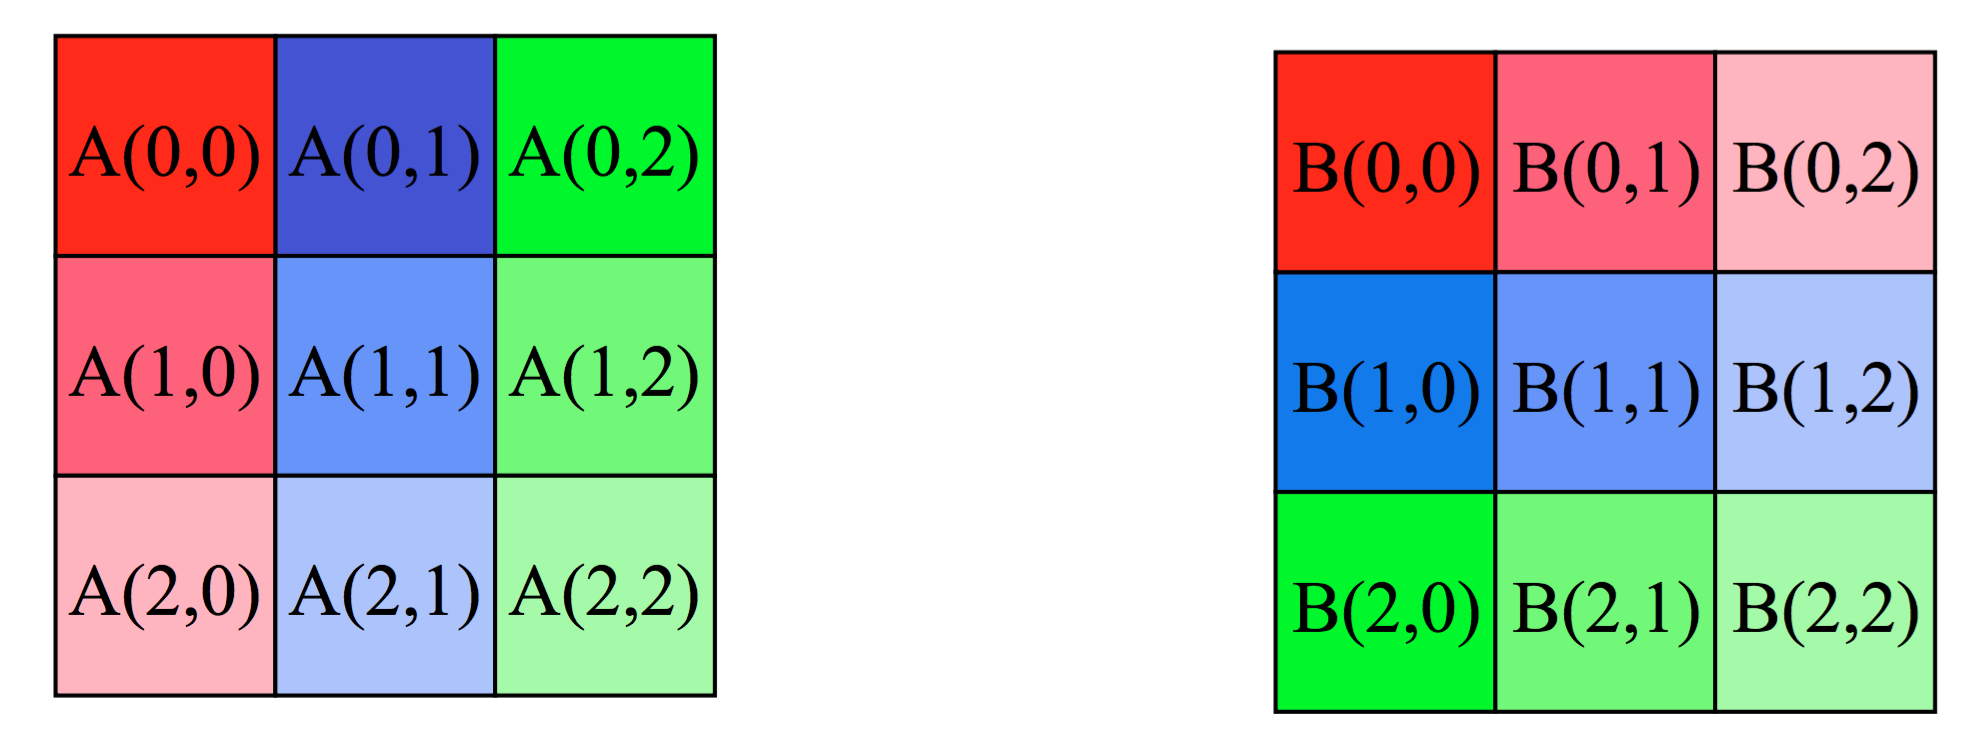
\includegraphics[width=10cm]{immagini/cannon1.png}
    \end{center}
    \caption{Cannon: matrici iniziali}
    \label{fig:cannon1}
\end{figure}

Vogliamo che A[1,0] e B[0,2] siano sullo stesso processo. Dunque sulla matrice A si fa uno shift delle righe (figura \ref{fig:cannon2}) e sulla matrice B si fa uno shift delle colonne (figura \ref{fig:cannon3}).

\begin{figure}[htbp]
    \begin{center}
        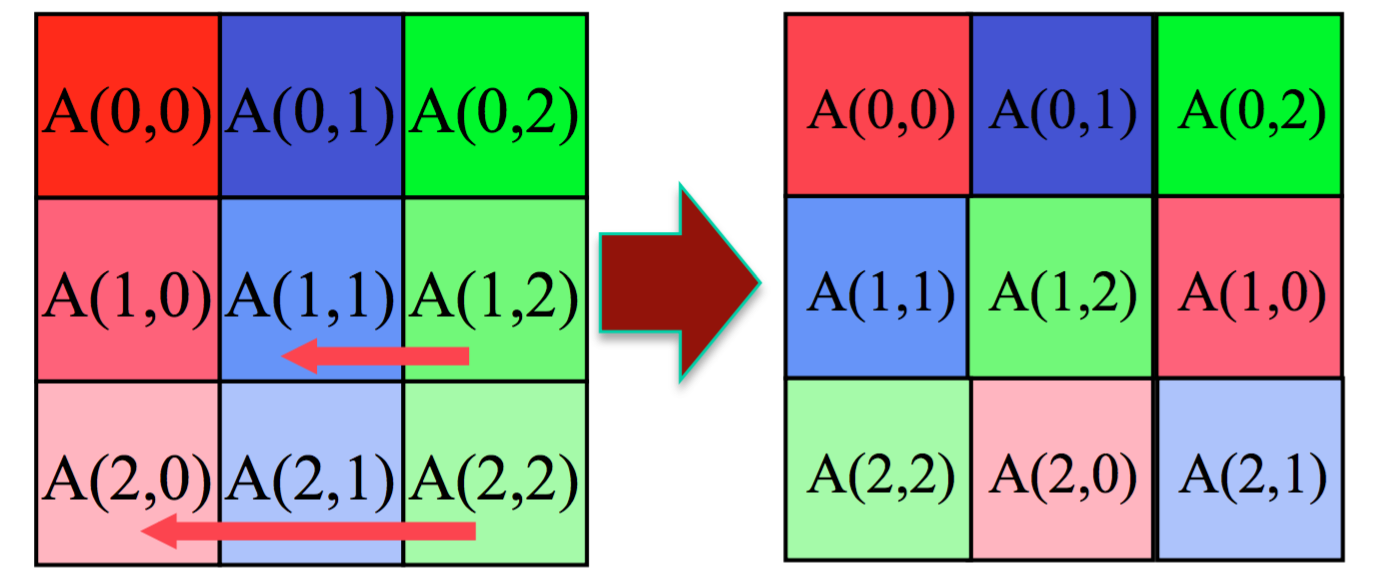
\includegraphics[width=10cm]{immagini/cannon2.png}
    \end{center}
    \caption{Cannon: shift iniziale sulla matrice A}
    \label{fig:cannon2}
\end{figure}

\begin{figure}[htbp]
    \begin{center}
        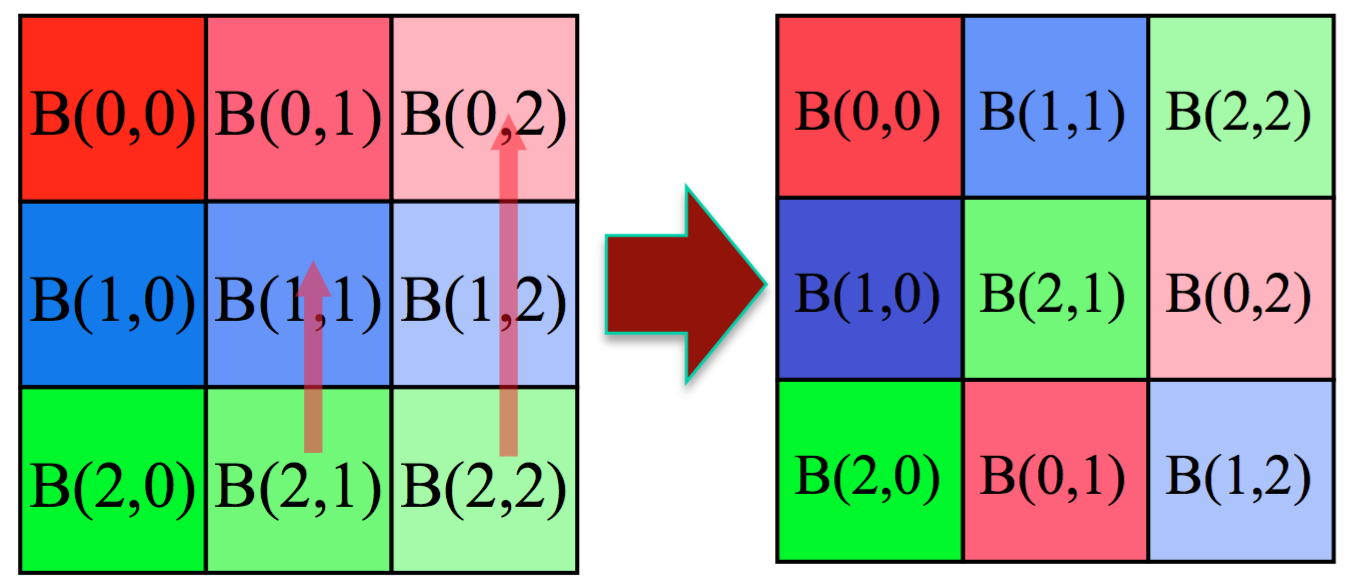
\includegraphics[width=10cm]{immagini/cannon3.png}
    \end{center}
    \caption{Cannon: shift iniziale sulla matrice B}
    \label{fig:cannon3}
\end{figure}

In questo modo si nota che la prossima coppia A[1,1] e B[1,2] sono pronti per essere spostati ed andare a finire dove A[1,0] e B[0,2] sono ora. La stessa cose si ripete per A[1,2] e B[2,2].

Appena effettuata la moltiplicazione possiamo effettuare un altro shift su tutte e due le matrici avendo le matrici come in figura \ref{fig:cannon4}. Come su pu\`{o} vedere, A[1,1] e B[1,2] sono allineati per essere moltiplicati.

\begin{figure}[htbp]
    \begin{center}
        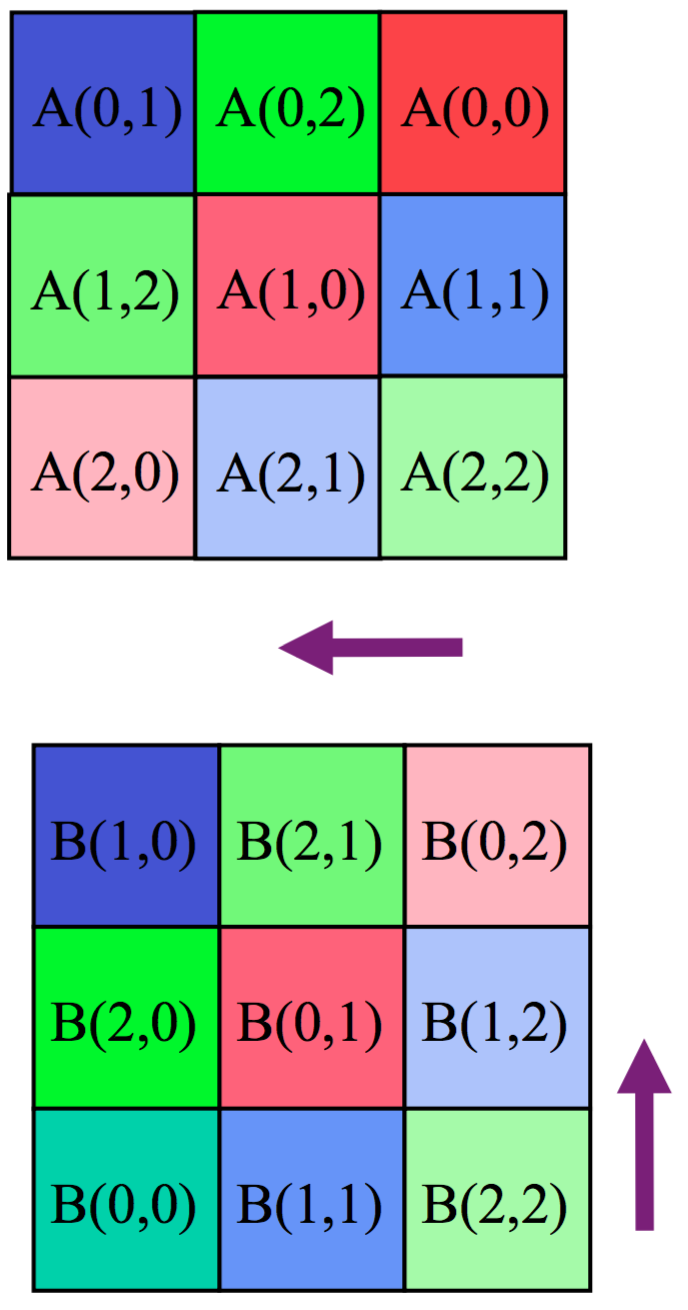
\includegraphics[width=5cm]{immagini/cannon4.png}
    \end{center}
    \caption{Cannon: shift sulle matrici A e B}
    \label{fig:cannon4}
\end{figure}

Si continua a shiftare in modo da avere A[1,2] e B[2,2] in posizione per effettuare la moltiplicazione.
